\documentclass{standalone}
\usepackage[T1]{fontenc}
\usepackage[utf8]{inputenc}
\usepackage{pgf,tikz}
\usetikzlibrary{calc}
\usepackage{pgfplots}
\usepackage[amssymb]{SIunits}


\begin{document}
  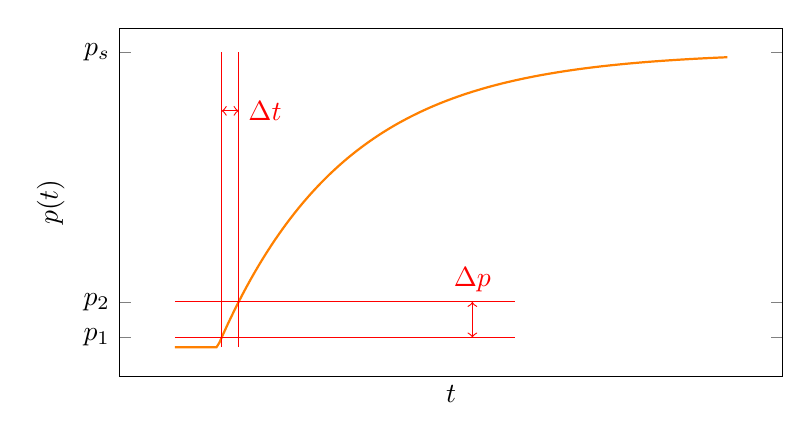
\begin{tikzpicture}[node distance=20mm]
     \def\Gain{1}
     \pgfmathsetmacro{\Timeconst}{300} % in ms
     \pgfmathsetmacro{\tone}{10} % 
     \pgfmathsetmacro{\ttwo}{50} %
     \pgfmathsetmacro{\pone}{\Gain * (1 - exp(-\tone/\Timeconst))} % 
     \pgfmathsetmacro{\ptwo}{\Gain * (1 - exp(-\ttwo/\Timeconst))} % 

     
     \pgfmathsetmacro{\xmax}{\Timeconst*4}
     \pgfmathsetmacro{\ucattc}{\Gain*0.632}

     %\node {\large \Timeconst};

     \begin{axis} [
       width=10cm,
       height=6cm,
       xlabel={$t$},
       ylabel={$p(t)$},
       xtick=\empty,
       ytick={\pone, \ptwo, \Gain},
       yticklabels={$p_1$, $p_2$, $p_s$},
       clip=false,
       ]
       
       \addplot+[thick, orange, no marks, domain=-100:\xmax, samples=200 ] {(x>0)*( \Gain * (1 - exp(-x/\Timeconst))};

       \draw[red] (axis cs: \tone, 0) to (axis cs: \tone, 1);
       \draw[red] (axis cs: \ttwo, 0) to (axis cs: \ttwo, 1);
       \draw[red, <->] (axis cs: \tone, 0.8) -- (axis cs: \ttwo, 0.8)  node[right] {$\Delta t$};
       \draw[red, ] (axis cs: -100, \pone) to (axis cs: 700, \pone);
       \draw[red, ] (axis cs: -100, \ptwo) to (axis cs: 700, \ptwo);
       \draw[red, <->] (axis cs: 600, \pone) -- (axis cs: 600, \ptwo) node[above] {$\Delta p$};
       % \draw[thick, red] (axis cs: \Timeconst, \ucattc) to (axis cs: \Timeconst, 0);
       %\node[coordinate, pin=180:{\ucattc}] at (axis cs: 0, \ucattc) {};
       %\node[coordinate, pin={[pin distance=10mm] -90:{\Timeconst}}] at (axis cs: \Timeconst, 0) {};

       
     \end{axis}
   \end{tikzpicture}
 \end{document}
 